\chapter{Ensayos y mediciones}

a. Medición de ripple.\\

  Para poder realizar las siguiente mediciones en este primer ensayo, previamente se realizo en la placa la soldadura del puente diodo y el filtro.\\

i. En el filtro capacitivo y determinación de parámetros.\\

  Se tomaran medidas de la tension tanto desde el punto bajo (desde 0 hasta 10 V) como desde el punto alto (desde 15 hasta 30 V) variando la corriente desde el vacio (0 A) hasta llegar a plena carga (1,5 A). Con las mediciones vamos a poder calcular los siguientes tres factores: Regulacion de voltaje, resistencia variable y factor de ripple.\\

Punto bajo:

  $V_{vacio} = 17,71 V$

  $V_{0,5A} = 15,80 V$
  
  $V_{0,75A} = 15,27 V$ 
  
  $V_{1A} = 14,63 V$
  
  $V_{1,25A} = 14,10V$
  
  $V_{PlenaCarga} = 13,69 V$\\

Para calcular la regulacion de voltaje se utiliza la siguiente formula:

$RV = \dfrac{V_{vacio} - V_{PlenaCarga}}{V_{PlenaCarga}} 100\percent $

$RV = \dfrac{17,71 - 13,69}{13,69} 100\percent = 29,36\percent $\\

La resistencia interna esta dada por:

$R_int = \dfrac{V_{PlenaCarga} - V_{vacio}}{-I_{carga}}$

$R_int = \dfrac{13,69 - 17,71}{-1,5} = 2,68\Omega $\\

Factor de ripple:

$F_R = \dfrac{V_{eficaz}}{V_{PlenaCarga}} 100\percent $

(completar)\\

\begin{figure}[H]
  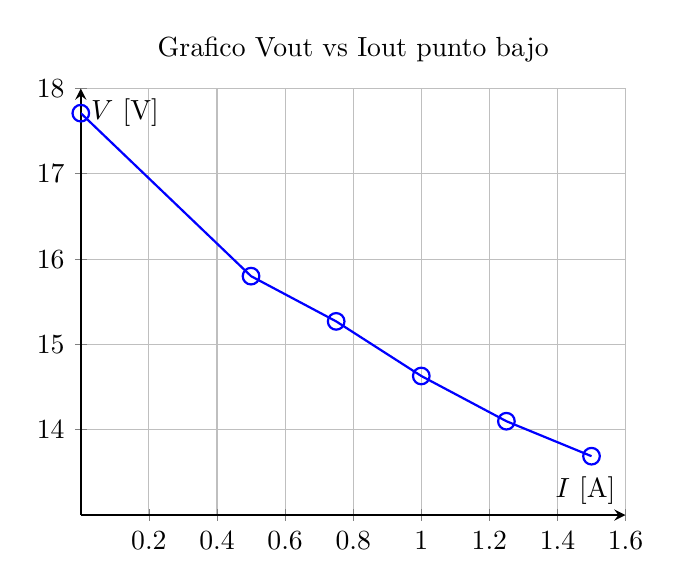
\begin{tikzpicture}
    \begin{axis}[
      axis lines = middle,
      xlabel = {$I$ [A]},
      ylabel = {$V$ [V]},
      domain = 0:1.5,
      samples = 200,
      grid = both,
      width=8.5cm,
      height=7cm,
      title = {Grafico Vout vs Iout punto bajo},
      xmin = 0, xmax= 1.6,
      ymin = 13, ymax = 18,
      thick
      ]
      \addplot[blue, mark=o, mark size=3pt] coordinates {
            (0, 17.71)
            (0.5, 15.80)
            (0.75, 15.27)
            (1, 14.63)
            (1.25, 14.10)
            (1.5, 13.69)
      };
    \end{axis}
  \end{tikzpicture}
\end{figure}


Punto alto: 
  $V_{vacio} = 36,68 V$

  $V_{0,5A} = 31,89 V$
  
  $V_{0,75A} = 31,05 V$ 
  
  $V_{1A} = 29,83 V$
  
  $V_{1,25A} = 28,55 V$
  
  $V_{PlenaCarga} = 27,43 V$\\

Regulacion de voltaje:

$RV = \dfrac{36,68 - 27,43}{27,43} 100\percent = 33,72\percent $\\

Resistencia interna:

$R_int = \dfrac{27,43 - 36,68}{-1,5} = 6,16\Omega $\\

Factor de ripple:

$F_R = \dfrac{}{} 100\percent $

(completar)\\

ii. Determinación de resistencia interna del transformador más la de los
diodos.

b. Mediciones finales

i. Regulación de voltaje

ii. Factor de ripple

iii. Cálculo de temperatura de juntura
